\chapter{Background}\label{chapter:background}
This chapter introduces \acrlong{abe} and the relevant mathematical background for implementing it.

\begin{figure} \centering
    \begin{subfigure}{.8\textwidth}
        \begin{tikzpicture}
            \draw[->] (0, 0) node [anchor=east] {m} -- ++(1, 0) node (encrypt) [anchor=west, draw] {Encrypt};
            \path (encrypt.north) -- +(0, 0.3) pic [anchor=west, scale=0.1, red, fill=red] {key};
            \draw[->] (encrypt.east) -- ++(2, 0) node [anchor=south] {c} -- ++(2,0) node (decrypt) [anchor=west, draw] {Decrypt};
            \path (decrypt.north) -- +(0, 0.3) pic [anchor=west, scale=0.1, red, fill=red] {key};
            \draw[->] (decrypt.east) -- ++(1,0) node [anchor=west] {m'};
        \end{tikzpicture}
        \caption{Symmetric Encryption: Both keys are identical.} \label{fig:keys-symmetric}
    \end{subfigure}
    \\
    \vspace{0.5cm}
    \begin{subfigure}{.8\textwidth}
        \begin{tikzpicture}
            \draw[->] (0, 0) node [anchor=east] {m} -- ++(1, 0) node (encrypt) [anchor=west, draw] {Encrypt};
            \path (encrypt.north) -- +(0, 0.3) pic [anchor=west, scale=0.1, olive, fill=olive] {key};
            \draw[->] (encrypt.east) -- ++(2, 0) node [anchor=south] {c} -- ++(2,0) node (decrypt) [anchor=west, draw] {Decrypt};
            \path (decrypt.north) -- +(0, 0.3) pic [anchor=west, scale=0.1, red, fill=red] {key};
            \draw[->] (decrypt.east) -- ++(1,0) node [anchor=west] {m'};
        \end{tikzpicture}
        \caption{Asymmetric Encryption: Different keys for encryption and decryption.} \label{fig:keys-asymmetric}
    \end{subfigure}
    \\ 
    \vspace{0.5cm}
    \begin{subfigure}{.8\textwidth}
        \begin{tikzpicture}[sibling distance=4mm, level distance=3mm]
            \draw[->] (0, 0) node [anchor=east] {m} -- ++(1, 0) node (encrypt) [anchor=west, draw] {Encrypt};
            
            \scoped{
                \tikzstyle{every node}=[fill, circle, draw, inner sep=0.5mm];
                \tikzstyle{level 2}=[sibling distance=1.5mm];
                \fill[red] (decrypt.north) -- ++(0, 0.7) node [anchor=south] {} child {node {} child {node {}} child {node {}} child {node {}}} child { node {} child {node {}}};
            };
            \draw[->] (encrypt.east) -- ++(2, 0) node [anchor=south] {c} -- ++(2,0) node (decrypt) [anchor=west, draw] {Decrypt};
            \path (encrypt.north) -- +(0, 0.3) node [olive] {$\{A, B, C\}$};
            \draw[->] (decrypt.east) -- ++(1,0) node [anchor=west] {m'};
        \end{tikzpicture}
        \caption{\glslink{gls-kp-abe}{Key-Policy Attribute-Based Encryption}: Attributes for encryption, access policy for decryption. Note that the access policy of the decryption key may be public; the actual key consists of secret shares that allow the user to decrypt a ciphertext if the correct attributes are present.} \label{fig:keys-abe}
    \end{subfigure}
    \caption[Keys in different classes of encryption schemes]{Keys used for encryption and decryption in different classes of encryption schemes. Red information has to be kept secret, green information may be made publicly available.}
    \label{fig:key-use}
\end{figure}

\section{Confidentiality with Classic Symmetric and Asymmetric Cryptography}
Today's conventional cryptography knows two main classes of cryptosystems: \glspl{privkes} and \glspl{pkes}. See Figure~\ref{fig:key-use} for an illustration of the differences.

Consider $n$ participants wanting to communicate securely (i.e. no user can read encrypted messages between two other users).
Using a \gls{privkes}, each participant would need to agree on a unique key with every other participant, resulting in a total number of $\frac{n(n-1)}{2}$ keys.
Using a \gls{pkes} reduces the number of keys to only $n$, because each participant could obtain everyone else's public key and then send messages to them securely.

Another problem remains, however: Encrypting a single message to a large number of participants requires encrypting it with everyone's public key separately.
For a large number of recipients, this is inefficient.
So, for example, to encrypt a message for all students of a certain university, we'd need to obtain each student's public key and encrypt the message with each key separately.

Even worse, what if we want to encrypt data for any student of said university, even if they \emph{haven't joined the university yet}.
In this case, our only option using classic public-key cryptography would be to have some trusted instance keep a plaintext copy and re-encrypt the data for any new student when they join the university.
Attribute-Based encryption solves this problem.

\section{Attribute-Based Encryption}
\acrfull{abe} uses a combination of attributes to define a \emph{group} of private keys that should be able to read encrypted data, instead of encrypting it for one specific private key only (as in \glspl{pkes}).
In Figure~\ref{fig:keys-abe}, this is represented by a tree.

The combination of attributes may be as restrictive or permissive as needed.
It is possible to create ciphertexts that can be read by almost all members of an \acrshort{abes}, and ciphertexts that can be read by nobody except a few selected participants.

Figure~\ref{fig:abe-system} shows a small \acrshort{abe} system with the \acrshort{kgc} initializing the system and issuing keys, and two users sharing an encrypted message.
\subsection{Attributes and the Key Generation Center}

\begin{figure}
    \centering
    \begin{subfigure}[t]{0.45\textwidth}
        \centering
        \begin{tikzpicture}[actor/.style={draw, minimum width=1.5cm}]
            \node[actor] (a) at (-1,0) {Alice};
            \node[actor] (b) at (1,0) {Bob};
            \node[actor] (kgc) at (0,1.5) {KGC};
        
            \node[above, align=center] at (kgc.north) {$\{PK, MK\}:=\text{Setup}()$};

            \node[below, align=center] at (a.south) {$\{m, \omega\}$\\};
            \node[below, align=center] at (b.south) {$\{\}$};

            % \draw[->] (a) edge node[left] {\{$S_A$\}} (kgc);
            % \draw[->] (b) edge node [right] {\{$S_B$\}} (kgc);
            % \draw[->] (a) edge pic [left=0.5cm, scale=0.05] {key} node [left=.5cm] {k} (kgc);
            \draw[->] (b) edge pic [right=0.5cm, scale=0.5, blue] {tree} node [right=.75cm, blue] {$S_B$} (kgc);
            \draw[->] (a) edge pic [left=0.5cm, scale=0.5, olive] {tree} node [left=.75cm, olive] {$S_A$} (kgc);
            % \draw[->] (b) edge node [right] {\{$S_B$\}} (kgc);

        \end{tikzpicture}
        \caption{The \acrshort{kgc} sets up the system and obtains Alice's and Bob's desired access policies.}
    \end{subfigure}
    ~~
    \begin{subfigure}[t]{0.45\textwidth}
        \centering
        \begin{tikzpicture}[actor/.style={draw, minimum width=1.5cm}]
            \node[actor] (a) at (-1,0) {Alice};
            \node[actor] (b) at (1,0) {Bob};
            \node[actor] (kgc) at (0,1.5) {KGC};

            \node[above, align=center] at (kgc.north) {$\{PK, MK\}$\\$\textcolor{olive}{k_A} := \text{KeyGen}(PK, MK, \textcolor{olive}{S_A})$\\$\textcolor{blue}{k_B} := \text{KeyGen}(PK, MK, \textcolor{blue}{S_B})$};

            \node[below, align=center] at (a.south) {{\{$PK$, $\textcolor{olive}{k_A}$\}}\\$\{m, \omega\}$};
            \node[below, align=center] at (b.south) {\{$PK$, $\textcolor{blue}{k_B}$\}};

            \draw[->] (kgc) edge pic [left=0.55cm, above=0.3cm, scale=0.05, olive] {key} node [left] {\{$PK$, $\textcolor{olive}{k_A}$\}} (a);
            \draw[->] (kgc) edge pic [right=1.1cm, above=0.3cm, scale=0.05, blue] {key} node [right] {\{$PK$, $\textcolor{blue}{k_B}$\}} (b);

            % \draw[->] (kgc) edge node [left] {\{$PK$, $\textcolor{olive}{k_A}$\}} (a);
            % \draw[->] (kgc) edge node [right] {\{$PK$, $\textcolor{blue}{k_B}$\}} (b);

        \end{tikzpicture}
        \caption{If $\textcolor{olive}{S_A}$ and $\textcolor{blue}{S_B}$ are allowed access policies for Alice and Bob, respectively, the \acrshort{kgc} creates their private keys and transmits them via a secure channel.}
    \end{subfigure}
    \par\bigskip
    \begin{subfigure}[c]{0.6\textwidth}
        \centering
        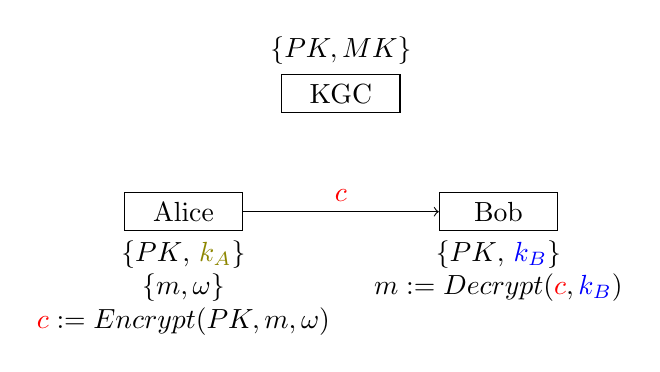
\begin{tikzpicture}[actor/.style={draw, minimum width=1.5cm}]
            \node[actor] (a) at (-2,0) {Alice};
            \node[actor] (b) at (2,0) {Bob};
            \node[actor] (kgc) at (0,1.5) {KGC};
        
            \node[above, align=center] at (kgc.north) {$\{PK, MK\}$};

            \node[below, align=center] at (a.south) {{\{$PK$, $\textcolor{olive}{k_A}$\}}\\$\{m, \omega\}$\\$\textcolor{red}{c}:=\text{Encrypt}(PK, m, \omega)$};
            \node[below, align=center] at (b.south) {\{$PK$, $\textcolor{blue}{k_B}$\}\\$m:=\text{Decrypt}(\textcolor{red}{c},\textcolor{blue}{k_B})$};
            % \node[below, align=center] at (a.south) {$\{PK, k_{A}\}$\\$\{m, \omega\}$};;
            % \node[below, align=center] at (b.south) {$\{PK, k_{B}\}$\\$m:=\text{Decrypt}(c,k_B)$};

            \draw[->] (a) edge node (c) [above] {$\textcolor{red}{c}$} (b);

            % \draw[->] (c.north) -- ++(0,.2) node [anchor=south] {\small $\omega$};
        \end{tikzpicture}
        \caption{Alice can now use the public parameters $PK$ and $\omega$ to encrypt a message for Bob, which he can decrypt only if his access policy $\textcolor{blue}{S_B}$ is satisfied by $\omega$. Note that the \acrshort{kgc} plays no role in this step}
    \end{subfigure}
    \caption[Interaction of Alice, Bob and KGC in an \acrshort{abes}]{
        Alice wants to send an \acrshort{kp-abe} encrypted message $m$ to Bob. She wants to encrypt the message under a set of attributes $\omega$.
        Both Alice and Bob create a desired Access Policy, $\textcolor{olive}{S_A}$ and $\textcolor{blue}{S_B}$, respectively.
        Note that the \acrshort{kgc} will only issue a corresponding key if it deems that they should be allowed to obtain a key under the given Access Policy.
    }
    \label{fig:abe-system}
\end{figure}
In essence, attributes are strings describing certain characteristics or features of actors and objects.
For example, a typical freshman student of informatics at TUM could be described by the attributes \texttt{"semester count 1", "computer science", "tum", "is young", "started degree in 2017"}.

These attributes themselves don't contain any information to which users or object they apply; instead this is a matter of interpretation.
Some attributes may be very clearly defined, e.g. \texttt{"started degree in 2017"} from above.
For others, it may be more difficult to decide whether they apply, e.g. the attribute \texttt{"is young"}: Until what age is a student young?

In any instance of \acrshort{abe}, there needs to exist an arbiter who decides whether an attribute applies to a certain user or object.
This role is assumed by a trusted third party, the \acrfull{kgc}.
It has two main responsibilities: First, the \acrshort{kgc} decides which attribute applies to which user.
Second, it issues private keys corresponding to these attributes, and hands these to the users.

Without this \acrshort{kgc}, there is no \acrshort{abe}.
This differs from traditional public-key encryption schemes, where any user can independently create their own keypair.

Regarding the \glsdesc{universe} (called the \emph{\gls{universe}}), there are two possibilities:
In a \gls{large-universe} construction, all possible strings can be used as attributes~\cite{goyal_attribute-based_2006}.
In a \gls{small-universe} construction, the universe of attributes is explicitly fixed when the system is instantiated, i.e. when the \acrshort{kgc} runs the \emph{Setup} algorithm (see below, section~\ref{sec:definition-es})~\cite{goyal_attribute-based_2006}.
With a \gls{small-universe} construction, the size of the public parameters usually grows with the size of the \gls{universe}~\cite{goyal_attribute-based_2006}.

\subsection{Formal definition of an ABE Scheme}\label{sec:definition-es}

We will define a \acrshort{kp-abe} scheme here, for the difference between \acrshort{cp-abe} and \acrshort{kp-abe} and formal definitions of Access Trees, see the next sections.

\begin{definition}
    A (Key-Policy) \Acrlong{abes} consists of the following four algorithms:~\cite{goyal_attribute-based_2006}
    \begin{itemize}
        \item \emph{Setup}. Run once by the \acrfull{kgc}. Sets up the system by generating public parameters $PK$ and a private master key $MK$. The public parameters are shared with all participants, while the master key remains only known to the \acrshort{kgc}.
        \item \emph{KeyGen(PK, s, S)}. Input: public parameters $PK$, master secret $s$ and Access Structure $S$.\\
        Run by the trusted authority once for each user to generate their private key. Returns a private key $k$ corresponding to $S$.
        \item \emph{Encrypt(PK, m, $\omega$)}. Input: public parameters $PK$, plaintext message $m$ and set of attributes $\omega$.\\
        Run by any participant of the system. Encrypts $m$ under $\omega$ and returns the ciphertext $c$.
        \item \emph{Decrypt(c, k)}. Input: ciphertext $c$ (output of \emph{Encrypt}) and key $k$ (output of \emph{KeyGen}).\\
        Run by any participant holding a private key generated by \emph{KeyGen}. Outputs the correctly decrypted message $m'$ if and only if the set of attributes under which $m$ was encrypted satisfies the access structure under which $k$ was created.
    \end{itemize}
\end{definition}

The definition of a \acrshort{cp-abe} scheme is identical, except that \emph{Encrypt(PK, m, S)} takes an Access Structure $S$ and \emph{KeyGen(PK, s, $\omega$)} takes a set of attributes.

How exactly these algorithms work in concrete ABE schemes will be discussed in Section~\ref{sec:concrete-schemes}.

\subsection{KP-ABE and CP-ABE}

Two components are necessary to specify a group of keys that shall be able to decrypt a ciphertext: A number of attributes that are present, and a policy that defines a combination of required attributes. 
Each of these can either be associated with the ciphertext, or with the decryption key:

In \acrfull{cp-abe}, so the key is associated with a set of attributes and the ciphertext is encrypted under an access policy.
\acrfull{kp-abe} works the other way around, so the ciphertext is associated with a set of attributes, and the key is associated with an access policy.
See Figure~\ref{fig:cp-kp-abe} for illustration.

In both cases, a ciphertext can be decrypted if and only if the set of attributes specified in one part satisfy the access policy associated with the other part.

\acrshort{cp-abe} tends to be more intuitive because, when encrypting a plaintext, the encryptor controls rather explicitly who can decrypt their ciphertext:
They set the access policy that defines which combinations of attributes are required from the users to successfully decrypt the ciphertext~\cite{bethencourt_ciphertext-policy_2007}.

With \acrshort{kp-abe}, on the other hand, the encryptor doesn't have any control over who will be able to access the data, except for the choice of attributes under which they encrypt the plaintext~\cite{bethencourt_ciphertext-policy_2007}.
Instead, the \acrlong{kgc} must be trusted with intelligently deciding which key to give to the decrypting party~\cite{bethencourt_ciphertext-policy_2007}.
For example, imagine a \acrshort{kp-abe} system in which it is common practice to label all ciphertexts with an attribute corresponding to the version number of the encryption software used.
If the \acrshort{kgc} were to give out a key containing an access structure with just a single attribute corresponding to a commonly-used version of this software, this key could be used to decrypt any ciphertext - completely disregarding any other attributes that might be associated with it.

An example use case for \acrshort{cp-abe} in a hospital setting would be sending an encrypted note about problems with a specific treatment to all doctors, patients that received that treatment and nurses of the department that administered the treatment.
This could be specified by an access policy as (\texttt{hospital-name} AND (\texttt{doctor} OR (\texttt{patient} AND \texttt{received-treatment-x}) OR (\texttt{nurse} AND \texttt{department-y})). % TODO maybe add a picture here

In the same hospital setting, \acrshort{kp-abe} could be employed in a different use case: When storing medical data about a patient, \acrshort{cp-abe} would require re-encrypting the data under a new access policy whenever a patient needs to see a different doctor.
With \acrshort{kp-abe}, the data could instead be associated with the patient's name as an attribute, and the hospital's IT department could extend the new doctor's key's policy to allow decrypting the new patient's data.

\begin{figure}
    \centering
    \begin{subfigure}[t]{0.4\textwidth}
        \begin{tikzpicture}
            % \fill (0, 0) -- +(0,0) arc (180:0:2) -- +(-0.5,0) arc (0:180:1.5) -- cycle;           
            % \fill[even odd rule] (0, 0) -- ++(0,3) -- ++(0.5,0) -- ++(0,1) arc (180:0:2) -- ++(0,-1) -- ++(0.5,0) -- ++(0,-3) -- cycle -- ++(1, 3) -- ++(0,1) arc (180:0:1.5) -- ++(0,-1) -- ++(-3,0);
            \path (0,0) node (ciphertext) {Ciphertext};
            \scoped[sibling distance=20, level distance=12, inner sep=2]{
                \tikzstyle{every node}=[fill, circle, draw];
                \tikzstyle{level 2}=[sibling distance=6];
                \fill[olive] (ciphertext.north) -- ++(0, 3) node (root) [anchor=south] {} child {node (b) {} child {node {}} child {node {}} child {node {}}} child { node {} child {node {}}};
            };  
            \path (ciphertext.north) ++(0, 0.5) pic [fill=olive, scale = 0.2] {lock};
            
            \path (2.5,0) node (key) {Key};
            \path (key.north) -- ++(0,2.5) node (atts) {\LARGE$\{A, B, C\}$};
            \path (key.north) -- ++(0,1) pic [scale=0.15] {key};
        \end{tikzpicture}
        \caption{CP-ABE}
    \end{subfigure}
    \begin{subfigure}[t]{0.4\textwidth}
        \begin{tikzpicture}
            % \fill (0, 0) -- +(0,0) arc (180:0:2) -- +(-0.5,0) arc (0:180:1.5) -- cycle;           
            % \fill[even odd rule] (0, 0) -- ++(0,3) -- ++(0.5,0) -- ++(0,1) arc (180:0:2) -- ++(0,-1) -- ++(0.5,0) -- ++(0,-3) -- cycle -- ++(1, 3) -- ++(0,1) arc (180:0:1.5) -- ++(0,-1) -- ++(-3,0);

            \path (2.5,0) node (key) {Key};
            \scoped[sibling distance=20, level distance=12, inner sep=2]{
                \tikzstyle{every node}=[fill, circle, draw];
                \tikzstyle{level 2}=[sibling distance=6];
                \fill (key.north) -- ++(0, 3) node (root) [anchor=south] {} child {node (b) {} child {node {}} child {node {}} child {node {}}} child { node {} child {node {}}};
            };  
            \path (key.north) -- ++(0,1) pic [scale=0.15] {key};
            
            \path (0,0) node (ciphertext) {Ciphertext};
            \path (ciphertext.north) -- ++(0,2.5) node (atts) [olive] {\LARGE$\{A, B, C\}$};
            \path (ciphertext.north) ++(0, 0.5) pic [fill=olive, scale = 0.2] {lock};
        \end{tikzpicture}
        \caption{KP-ABE}
    \end{subfigure}
    \caption[\acrshort{cp-abe} vs. \acrshort{kp-abe}]{\acrshort{cp-abe} vs. \acrshort{kp-abe}: Association of key and ciphertext with Access Policy and set of attributes.}
    \label{fig:cp-kp-abe}
\end{figure}

\subsection{Access Trees}

\begin{figure}
    \centering
    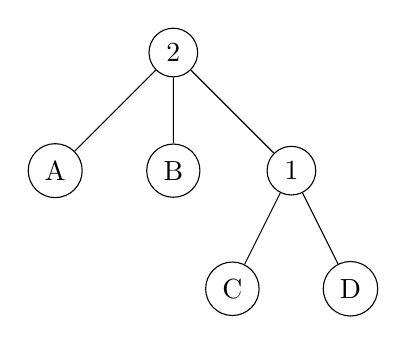
\begin{tikzpicture}
        \scoped{
                \tikzstyle{every node}=[circle, draw];
                \draw (0,0) node (root) [anchor=south] {2} child {node (a) {A}} child {node (b) {B}} child  {node (subroot) {1} child  {node (c) {C}} child  {node (d) {D}}};
            };
    \end{tikzpicture}
    \caption[Sample Access Tree]{
        Sample Access Tree over the attributes \texttt{A}, \texttt{B}, \texttt{C}, \texttt{D}.
    }
    \label{fig:sample-access-tree}
\end{figure}
Of course, we need a way to define the access policies associated with the key (KP-ABE) or the ciphertext (CP-ABE), respectively.
For this, we will use the construction of \emph{Access Trees} from Goyal~et~al. in~\cite{goyal_attribute-based_2006}.
Each leaf of this tree is labelled with an attribute, and each interior node is labelled with an integer, the threshold for it to be satisfied~\cite{goyal_attribute-based_2006}.

Figure~\ref{fig:sample-access-tree} illustrates an example for an Access Tree. It is satisfied by any set of attributes that contains two of $A, B$ and either $C$ or $D$.
That is, $\{A,B\}$ would satsify the tree, just as $\{B, D\}$ would, but $\{C, D\}$ would not be sufficient.

\begin{definition}
    Access Tree~\cite{goyal_attribute-based_2006}.\\
    An interal note $x$ of an access tree is defined by its children and a threshold value $d_x$. If $x$ has $num_x$ children, then its threshold value satisfies $0 < d_x \leq num_x$.\\
    A leaf node $x$ is defined by an attribute and a threshold value $k_x = 1$.

    \cite{goyal_attribute-based_2006} also defines the following functions for working with access trees:
    The parent of a node $x$ in the access tree is denoted by $\text{parent}(x)$.
    If $x$ is a leaf node, $\text{att}(x)$ denotes the attribute associated with $x$; otherwise it is undefined.
    The children of a node $x$ are numbered from $1$ to $num_x$. Then $\text{index}(y)$ denotes the unique index of $y$ among the children of its parent node.
\end{definition}

\begin{definition}
    Satisfying Access Trees~\cite{goyal_attribute-based_2006}.\\
    Let $\mathcal{T}$ be an access tree with root r and $\mathcal{T}_x$ the subtree with $x$ as its root.
    If a set of attributes $\gamma$ satisfies the access tree $\mathcal{T}_x$, we write $\mathcal{T}_x(\gamma) = 1$; otherwise $\mathcal{T}_x(\gamma) = 0$.\\
    If $x$ is a leaf node, then $\mathcal{T}_x(\gamma) = 1$ if and only if $\text{attr}(x) \in \gamma$.\\
    If $x$ is an internal node, then $\mathcal{T}_x = 1$ if and only if $d_x$ or more of the children $x'$ of $x$ return $\mathcal{T}_{x'}(\gamma) = 1$.
\end{definition}

Using this construction with threshold gates, we can express \emph{A AND B} as a node with two children $A$ and $B$ and threshold $2$, and express \emph{A OR B} as a node with two children $A$ and $B$ and threshold $1$~\cite{yao_lightweight_2015}.

\section{Shamir's Secret Sharing}
This secret sharing scheme based on polynomial interpolation was first introduced by Adi Shamir in 1979~\cite{shamir_how_1979}.
It allows a secret $s$, which is generally just a number, to be shared among a number of $n$ participants.
The shares are computed such that $s$ can be reconstructed if, and only if, at least $k$ participants meet and combine their shares.
Such a theme is then called a $(k,n)$-threshold scheme.~\cite{shamir_how_1979}

\subsection{Lagrange interpolation}
Shamir's scheme makes use of a property of polynomials: A polynomial of degree $d$ is unambiguously determined by $d+1$ points $(x_i, y_i)$.
In other words, any polynomial of degree $d$ can be unambiguously interpolated (reconstructed) from $d+1$ distinct points.

To interpolate a polynomial of degree $d$ from $d+1$ given points $(x_1, y_1), \dots, (x_{d+1}, y_{d+1})$, we can make use of the lagrange basis polynomials:~\cite{yao_lightweight_2015}

\begin{definition}
    Lagrange interpolation: Given a set of $d+1$ points $(x_1, y_1), \dots, (x_{d+1}, y_{d+1})$.

    Then the polynomial 
    \begin{equation}
        L(x) = \sum_{k=0}^d l_{\omega, x_k}(x) \cdot y_k
    \end{equation}
    is the lagrange interpolation polynomial for that set of points, where $\omega = \{x_1, \dots, x_{d+1}\}$ and $l_{\omega,k}(x)$ are the Lagrange basis polynomials:
    \begin{equation}
        l_{\omega,k}(x) = \prod_{\substack{i\in\omega\\ i \neq k}}^d \frac{x-i}{k-i}
    \end{equation}
\end{definition}

This polynomial has degree $d$. If the points $(x_i, y_i)$ lie on a $d$-degree polynomial, then the lagrange interpolation $L(x)$ is \emph{exactly} that polynomial.

On the other hand, if there are less than $d+1$ points of a $d$-degree polynomial known, there are infinitely many $d$-degree polynomials that pass through all given points.~\cite{shamir_how_1979}

% The polynomial can be interpolated unambiguously if at least $k$ points are known, because it has degree $k-1$.
% If only $k-1$ points (or less) are known, there are infinitely many ways to construct a polynomial that passed through all $k-1$ points.
% Therefore, then there are also infinitely many possibilities for $s$.

\subsection{Secret sharing with polynomials}
To share our secret, we now hide it in a polynomial and give out points on this polynomial as secret shares.
Using the lagrange basis polynomials, we can then reconstruct $p(x)$ and thus the secret if we know enough shares.~\cite{shamir_how_1979}

\begin{figure}
    \centering
    \begin{tikzpicture}
        \begin{axis} [axis lines=center, xlabel=$x$, ylabel=$p(x)$, ymin=0]
            \addplot [domain=-0.1:5.05, smooth, thick, color=red] { \PolynomialSSS(x)};
            \fill (axis cs:0,\PolynomialSSS(0)) circle [radius=2pt] node [right] {(0,~s)};
            \fill[color=ForestGreen] (axis cs:1,\PolynomialSSS(1)) circle [radius=2pt] node [right] {(1,~10)};
            \fill[color=ForestGreen] (axis cs:2,\PolynomialSSS(2)) circle [radius=2pt] node [right] {(2,~6)};
            \fill[color=ForestGreen] (axis cs:3,\PolynomialSSS(3)) circle [radius=2pt] node [above] {(3,~2)};
            \fill[color=ForestGreen] (axis cs:4,\PolynomialSSS(4)) circle [radius=2pt] node [right] {(4,~4)};
            \fill[color=ForestGreen] (axis cs:5,\PolynomialSSS(5)) circle [radius=2pt] node [left] {(5,~18)};
          \end{axis}
    \end{tikzpicture}
    \caption[Plot of $(5,4)$-threshold secret sharing scheme]{
        Example for a $(5, 4)$-threshold scheme with $s=8$ and $p(x) = 8 + 7x - 6x^2 + x^3$.
        The five green-colored points are distributed as the secret shares.
        As $p(x)$ has degree three, at least four shares are required to reconstruct $s$.
    }
    \label{fig:sss}
\end{figure}

\begin{definition}
    Shamir's $(k, n)$-threshold secret sharing scheme~\cite{shamir_how_1979}.
    To share a secret $s$ among $n$ participants such that $s$ can be recovered if and only if $k$ or more shares are combined, do:
    \begin{enumerate}
        \item Pick coefficients $a_1, ..., a_{k-1}$ at random 
        \item Set $a_0 = s$. This results in the polynomial $p(x) = a_0 + a_1x + \cdots + a_{k-1}x^{k-1}$. Note that $p(0) = s$.
        \item The secret shares are $(1, p(1)), (2, p(2)), \dots, (n, p(n))$. Give one to each participant.
    \end{enumerate}
    To reconstruct the secret from any subset of $k$ shares, interpolate the polynomial $p(x)$ and evaluate $p(0) = s$. 
\end{definition}

See also Figure~\ref{fig:sss} for illustration.
In practice, the numbers would be far bigger and calculations wouldn't be performed over the real numbers, but rather a finite field modulo a prime.~\cite{shamir_how_1979}

\subsection{Secret Sharing in Attribute Based Encryption}
To realize an Access Tree that ,,gives away'' a secret if and only if it is satsified by a set of attributes, we can recursively use Shamir's Secret Sharing scheme:

\begin{figure}
    \centering
    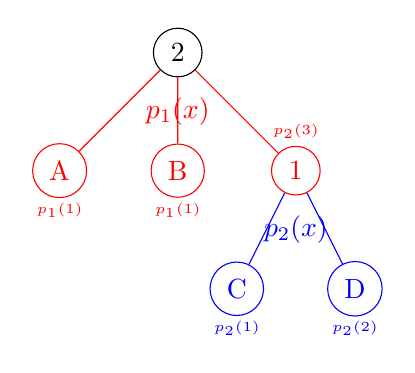
\begin{tikzpicture}
        \scoped{
                \tikzstyle{every node}=[circle, draw];
                \draw (0,0) node (root) [anchor=south] {2} child [red] {node (a) {A}} child [red] {node (b) {B}} child [red] {node (subroot) {1} child [blue] {node (c) {C}} child [blue] {node (d) {D}}};
            };
            \path[red] (root) -- +(0, -0.75) node {$p_1(x)$};
            \path[red] (a) -- +(0, -0.5) node {\tiny$p_1(1)$};
            \path[red] (b) -- +(0, -0.5) node {\tiny$p_1(1)$};
            \path[red] (subroot) -- +(0, 0.5) node {\tiny$p_2(3)$};

            \path[blue] (subroot) -- +(0, -0.75) node {$p_2(x)$};
            \path[blue] (c) -- +(0, -0.5) node {\tiny$p_2(1)$};
            \path[blue] (d) -- +(0, -0.5) node {\tiny$p_2(2)$};
    \end{tikzpicture}
    \caption[Shamir's Secret sharing in Access Trees]{
        Access Tree from Figure~\ref{fig:sample-access-tree} showing how Shamir's Secret Sharing is employed recursively.
        $p_1(x)$ is a the polynomial of a $(2,3)$-threshold scheme, $p_2(x)$ of a $(1,2)$-threshold scheme.
        Shown in small are the secret shares embedded into each node.
    }
    \label{fig:sample-access-tree-shamir}
\end{figure}

Quite simplified, we now employ Shamir's Secret Sharing Scheme recursively on each internal node of the Access Tree:
For a node $x$ with threshold $d_x$ and $\text{num}_x$ children, we define a $(d_x, \text{num}_x)$-threshold scheme and embed one share of the secret in each child.
Begin in the root, and set $s$ as the secret we want to embed in the tree. For all other nodes, set $s$ as the secret share received from the parent node.

If the child is a leaf, we modify the share such that it can only be used if the relevant attribute is present (we will not discuss how this is done at this point).

Now, let $\omega$ be a set of attributes.
We have built our tree in such a way that the share embedded in a leaf node $u$ can be used only if $\text{attr}(u) \in \omega$.
That means, a leaf node's secret share can be used if and only if the set of attributes satisfies this leaf node.

For the internal nodes $x$, the use of a $(d_x, \text{num}_x)$-threshold scheme ensures that the secret embedded in $x$ can be reconstructed if and only if the secret shares of at least $d_x$ child nodes can be used, i.e. at least $d_x$ child nodes are satisfied.
Following this recursive definition up to the root, we can see that our secret $s$ embedded in the root can be reconstructed exactly if $\omega$ satisfies the Acess Tree.

See Figure~\ref{fig:sample-access-tree-shamir} for an illustration with the tree from Figure~\ref{fig:sample-access-tree}:
Two $(k,n)$-threshold schemes are employed, one for each internal node of the access tree.
$p_1(x)$ is the polynomial of the root's $(2,3)$-threshold scheme, sharing $s$, the secret to be embedded in the tree (i.e. $p_1(0) = s$).
$p_2(x)$ is the polynomial for the $(1,2)$-threshold scheme belonging to the node labelled ``1'' and shares the value $p_1(3)$ that it received from the $(2,3)$-threshold scheme of the layer above (i.e. $p_2(0) = p_1(3)$).

\section{Elliptic Curves}
\label{sec:ec}

The mathematics of modern cryptosystems (including, but not limited to ABE) work any group that satisfies the axioms (see below), and elliptic curves are just one of them.
Because \Glspl{ec} allow for shorter key lengths than, e.g. groups modulo a prime, they have become very popular for use in cryptography.
Exact definitions and notations differ, these are taken from the textbook \emph{Introduction to Modern Cryptogaphy} by Katz and Lindell~\cite{katz_introduction_2015}.

\subsection{Group Axioms}\label{sec:group}
\begin{definition}~\cite{katz_introduction_2015}. A \emph{Group} consists of a set $\mathbb{G}$ together with a binary operation $\circ$ for which these four conditions hold:
    \begin{itemize}
        \item Closure: For all $g, h \in \mathbb{G}$, $g \circ h \in \mathbb{G}$.
        \item Existence of identity: There is an element $e \in \mathbb{G}$, called the \emph{identity}, such that for all $g \in \mathbb{G}$, $g \circ e = g = e \circ g$.
        \item Existence of inverse: For every $g \in \mathbb{G}$ there exists an \emph{inverse} element $h \in \mathbb{G}$ such that $g \circ h = e = h \circ g$.
        \item Associativity: For all $g_1, g_2, g_3 \in \mathbb{G}$, $(g_1 \circ g_2) \circ g_3 = g_1 (\circ g_2 \circ g_3)$.
    \end{itemize}
    When $\mathbb{G}$ has a finite number of elements, the group $\mathbb{G}$ is called finite and $|\mathbb{G}|$ denotes the order of the group.

    A group $\mathbb{G}$ with operation $\circ$ is called \emph{abelian} or commutative if, in addition, the following holds:
    \begin{itemize}
        \item Commutativity: For all $g, h \in \mathbb{G}, g \circ h = h \circ g$.
    \end{itemize}

    When the binary operation is clear from context, we simply use $\mathbb{G}$ to denote the group.

    We also define \emph{Group Exponentiation}: $g \in \mathbb{G}, m \in \mathbb{N}^+$, then $mg = \underbrace{g \circ \cdots \circ g}_{m \text{ times}}$.
\end{definition}

Usually, the symbol used to denote the group operation is not the $\circ$ from above, but either $+$ or $\cdot$. These are called \emph{additive} and \emph{multiplicative} notation, respectively.
It is important to remember, though, that the group operation might be defined completely differently!

In multiplicative notation, the group exponentiation of $g \in \mathbb{G}$ with $m \in \mathbb{N}^+$ is written as $g^m$, in additive groups it is written as $m \cdot g$.

\subsection{Elliptic Curves}

\begin{definition}
    Given a prime $p \geq 5$ and $a, b \in \mathbb{Z}_p$ with $4a^2 + 27b^2 \neq 0 \bmod{p}$, the Elliptic Curve over $\mathbb{Z}_p$ is:~\cite{katz_introduction_2015}
    \begin{equation}
        E(\mathbb{Z}_p) := \{(x, y)~|~x,y \in \mathbb{Z}_p \text{ and } y^2 = x^3 + a x + b \bmod{p}\} \cup \{\mathcal{O}\}
    \end{equation}
\end{definition}

$a$ and $b$ are called the curve parameters, and the requirement that $4a^2 + 27b^2 \neq 0 \bmod{p}$ makes sure that the curve has no repeated roots~\cite{katz_introduction_2015}.
The curve is simply the set of points $(x, y) \in \mathbb{Z}_p \times \mathbb{Z}_p$ that satisfy the curve equation $y^2 = x^3 + a x + b \bmod{b}$.
One special point is added, the \emph{point at infinity} denoted by $\mathcal{O}$. This will help define the point addition as a group operation in the next paragraph.~\cite{katz_introduction_2015}

\subsection{Point Addition}
Now, it is possible to show that every line intersecting a curve $E(\mathbb{Z}_p)$ intersects it in exactly three points, if you (1) count tangential intersections double and (2) count any vertical line as intersecting the curve in the point at infinity $\mathcal{O}$~\cite{katz_introduction_2015}.
Therefore, $\mathcal{O}$ can be thought of as sitting ``above'' the end of the y-axis~\cite{katz_introduction_2015}.
Figure~\ref{fig:ecc-point-addition} shows all four different combinations, feel free to convince yourself that this statement indeed makes sense for the plotted curve.

Using this intersecting line, we can define an operation on curve points:
\begin{definition}
    \label{def:point-add}
    Given an Elliptic Curve $E(\mathbb{Z}_p)$, we define a binary operation called \emph{(point) addition} and denoted by $+$:~\cite{katz_introduction_2015}\\
    Let $P_1, P_2 \in E(\mathbb{Z}_p)$.

    \begin{itemize}
        \item For two points $P_1, P_2 \neq \mathcal{O}$ and $P_1 \neq P_2$, their sum $P_1 + P_2$ is evaluated by drawing the line through $P_1$ and $P_2$. 
            This line will intersect the curve in a third point, $P_3 = (x_3, y_3)$.
            Then the result of the addition is $P_1 + P_2 = (x_3, -y_3)$, i.e. $P_3$ is reflected in the $x$-axis (Figure~\ref{fig:ecc-point-addition}-1).
            If $P_3 = \mathcal{O}$, then the result of the addition is $\mathcal{O}$ (Figure~\ref{fig:ecc-point-addition}-3).
        \item If $P_1, P_2 \neq \mathcal{O}$ and $P_1 = P_2$, as above but draw the line as tangent on the curve in $P_1$ (Figure~\ref{fig:ecc-point-addition}-2 and -4).
        \item If $P_1 = \mathcal{O}$, then $P_1 + P_2 = P_2$ and vice-versa.
    \end{itemize}
\end{definition} 

\begin{figure}
    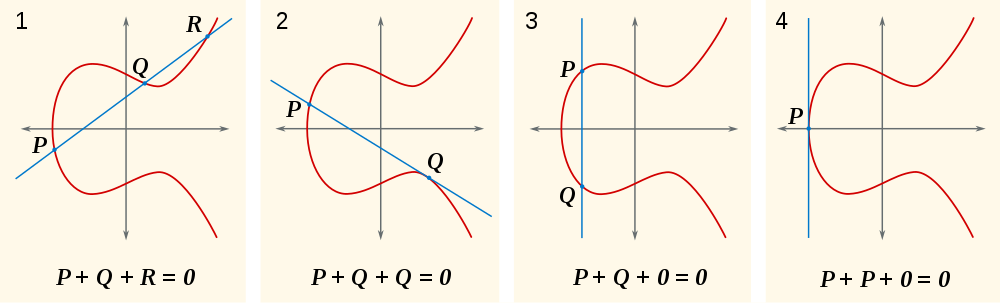
\includegraphics[width=\textwidth]{figures/ecc_point_addition.png}
    \caption[Elliptic Curve point addition]{Elliptic Curve point addition\\(Image by \href{https://commons.wikimedia.org/wiki/File:ECClines-2.svg}{SuperManu}, licensed under \href{https://creativecommons.org/licenses/by-sa/3.0/deed.en}{Creative Commons}.)}
    \label{fig:ecc-point-addition}
\end{figure}

We will be adding points to themselves a lot. Therefore, we define for ease of notation:
\begin{definition}
    Point-Scalar multiplication: Given a point $P \in E(\mathbb{Z}_p)$ and a scalar $d \in \mathbb{N}$: 
    \begin{equation}
        d \cdot P = \underbrace{P + P + \cdots + P}_{d \text{ times}}
    \end{equation}
\end{definition}
 
That is exactly the definition of group exponentiation, applied to our additive \Gls{ec} group. Note that the product of a scalar with a point is again a point on our curve.
\\

\subsection{Groups on Elliptic Curves}
\begin{theorem}
    The points of an Elliptic Curve $E(\mathbb{Z}_p)$ plus the addition law as stated in Definition~\ref{def:point-add} forms an abelian (commutative group)~\cite{katz_introduction_2015, washington_elliptic_2008}:
\end{theorem}
\begin{proof}
    A formal proof is outside the scope of this thesis, but here's some informal reasoning about the group axioms:
    \begin{itemize}
        \item Existence of Identity: $P + \mathcal{O} = P$ (as per definition)
        \item Commutativity: For all $P_1, P_2 \in E(\mathbb{Z}_p)$, $P_1 + P_2 = P_2 + P_1$ (obvious, because the line through $P_1$ and $P_2$ will be the same)
        \item Unique inverse: For any point $P = (x,y) \in E(\mathbb{Z}_p)$, the unique inverse is $-P = (x, -y)$ (obvious).
        \item Associativity: For all $P_1, P_2, P_3 \in E(\mathbb{Z}_p)$, $(P_1 + P_2) + P_3 = P_1 + (P_2 + P_3)$ (much less obvious, see e.g.~\cite[Chapter 2.4]{washington_elliptic_2008} for a proof).
    \end{itemize}
\end{proof}

Of particular interest to cryptography are \emph{cyclic} groups on elliptic curves:
\begin{definition}
    A (multiplicative) group $\mathbb{G}$ is cyclic if there is an element $g \in \mathbb{G}$ that generates $\mathbb{G}$, i.e. $\mathbb{G} = \langle g \rangle = \{g^n | n \in \mathbb{Z}\}$.
\end{definition}

Translated to our (additive) groups on elliptic curves, this means that there is a generator point $P \in E(\mathbb{Z}_p)$, such that every point $Q \in E(\mathbb{Z}_p)$ can be written as $Q = nP$ with some $n \in \mathbb{N}$.

\begin{theorem}\cite{katz_introduction_2015}
    Let $\mathbb{G}$ be a finite group of order $n$, i.e. $|\mathbb{G}| = n$.
    Let $g \in \mathbb{G}$ be an element of $\mathbb{G}$ with order $k$, i.e. $k = |\langle g \rangle |$

    Then $k|n$, i.e. the order of $g$ divides the group order $n$.
\end{theorem}
\begin{proof}
    See \cite*[Proposition 8.54]{katz_introduction_2015}.
\end{proof}

There is an important consequence to this fact: If a group has prime order, all points except the identity are generators.
This stems from the fact that a prime number has exactly two divisors: One (the order of the identity) and itself (the order of all other points).
\\
This follows from the fact that for any point $P \in E(\mathbb{Z}_p)$, its order $\text{ord}(P) = | \langle P \rangle |$ must divide the group order.
A prime has exactly two divisors: One (the order of $\mathcal{O}$) and itself (the order of all other points).

Again, translated to Elliptic Curves this means that if the number of points $\#E(\mathbb{Z}_p)$ on a curve is prime, all points except $\mathcal{O}$ are generators.
These cyclic elliptic curve groups (or, cyclic subgroups of non-cyclic elliptic curves) are exactly the groups we are interested in for doing actual cryptography. For a detailed description why, see \cite[p.~321]{katz_introduction_2015}.

\subsection{Hardness Assumptions}

Most ECC schemes are build upon three hardness assumptions: The Discrete Logarithm Problem (DLP), the Decisional Diffie-Hellman Problem (DDHP) and the Computational Diffie-Hellman Problem (CDHP).
Given an additive, cyclic group $\mathbb{G}$ with $P \in \mathbb{G}$ a generator, they are stated as follows:
\\

\emph{Discrete Logarithm Problem.} Given an arbitrary point $Q \in \mathbb{G}$, compute an $n \in \mathbb{N}$ such that $n P = Q$. % n from Zq?

\emph{Computational Diffie-Hellman Problem.} Given the triple $(P, aP, bP)$ where $a, b \in \mathbb{N}$ chosen uniformly at random, compute $abP$.

\emph{Decisional Diffie-Hellman Problem.} Given two triples $(aP, bP, abP)$ and $(aP, bP, Q)$ where $a, b \in \mathbb{N}$ and $Q \in \mathbb{G}$ chosen uniformly at random, distinguish between the two.
\\

Now, the hardness \emph{assumption} is that, for some groups, these problems are hard to solve, i.e. solving them requires so much time and computational power that it is infeasible.
From this, we can build secure asymmetric encryption schemes.

These three problems might all be assumed to be \emph{hard}, but that doesn't mean they are equally so:
If, in a certain group $\mathbb{G}$, the DLP problem is easy, so is CDHP: Just compute $a$ and $b$, and then use them to calculate $abP$.
And if CDHP is easy w.r.t some $\mathbb{G}$, so is DDHP: Just compute $abP$, and compare the third element of each tuple.
The inverse is not generally true, i.e. there are groups in which DLP and CDHP are hard to solve, even though DDHP is easy to solve.
In that sense, DLP is the hardest and DDHP the easiest of the three. \cite{katz_introduction_2015} (TODO find out if this is true. \cite{menezes_introduction_2009})

\subsection{Bilinear Pairings}
\subsubsection{Introduction}
The final primitive needed for pairing-based encryption schemes are bilinear pairings. These are functions mapping two points on (possibly different) elliptic curves to elements of a finite field (\emph{not} another point on a curve).\cite{blake_advances_2005}

Let $n \in \mathbb{N}_0$, $\mathbb{G}_1$ denote an additive abelian group of order $n$ with generator $P$ and identity $\mathcal{O}$. 
Let $\mathbb{G}_T$ be another group of order $n$, this time written multiplicatively with generator $g$ and identity $1$.
A \emph{bilinear pairing} then is a function $e: \mathbb{G}_1 \times \mathbb{G}_1 \rightarrow \mathbb{G}_T$ with the following properties:
\begin{itemize}
    \item \emph{Bilinearity.} For all $Q_1, Q_2, Q_3 \in \mathbb{G}_1$, $e(Q_1+Q_2, Q_3) = e(Q_1,Q_3)+e(Q_2,Q_3)$ and $e(Q_1, Q_2+Q_3)=e(Q_1,Q_2)+e(Q_1,Q_3)$
    \item \emph{Non-Degeneracy.} $e(P,P) \neq 1$
\end{itemize}

Using a bilinear pairing with a group $\mathbb{G}_T$ where the DLP is easy to solve, the DLP in $\mathbb{G}_1$ can also be solved easily:
To find $n$ such that $Q = nP$, compute $e(P,Q) = e(P, nP) = e(P, \underbrace{P+\cdots+P}_{n \text{ times}}) = \underbrace{e(P,P) \cdots e(P,P)}_{n \text{ times}} = e(P,P)^n$.
Thus, the discrete logarithm of $Q$ with respect to $P$ is the discrete logarithm of $e(P,Q)$ with respect to $g = e(P,P) \in \mathbb{G}_T$.~\cite{menezes_introduction_2009}

\subsubsection{Bilinear Hardness Assumption}

Since the DLP can be easy to solve using pairings, we need to adapt our hardness assumption. Therefore, we define

The \emph{Bilinear Diffie-Hellman Problem} (BDHP): Given $P, aP, bP, cP$ with $a,b,c \in \{1,\dots,n-1\}$ chosen randomly, compute $e(P, P)^{abc}$.~\cite{menezes_introduction_2009}

If the BDHP is hard for a pairing $e$ on groups $\mathbb{G}_1 \text{ and } \mathbb{G}_T$, this implies that the DLP is hard in both $\mathbb{G}_1 \text{ and } \mathbb{G}_T$.~\cite{menezes_introduction_2009}

\section{Different ABE schemes for use in Embedded Devices}\label{sec:concrete-schemes} 
\subsection{Yao, Chen and Tian 2015}

This scheme was described by Yao, Chen and Tian \cite{yao_lightweight_2015} in 2015.
In 2019, Tan, Yeow and Hwang \cite{tan_enhancement_2019} proposed an enhancement, fixing a flaw in the scheme and extending it to be a hierarchical KP-ABE scheme. %TODO explain what that is.

Yao, Chen and Tian's ABE scheme (hereafter written just YCT) is a KP-ABE scheme that does not use any bilinear pairing operations.
Instead, the only operation performed on Elliptic Curves are point-scalar multiplication~\cite{yao_lightweight_2015}.
This makes it especially useful for our resource-constrained context, as bilinear pairings are significantly more costly in terms of computation and memory.

As opposed to other ABE schemes based on pairings, YCT uses a hybrid approach similar to Elliptic Curve Integrated Encryption Standard (ECIES):
The actual encryption of the plaintext is done by a symmetric cipher, for which the key is derived from a curve point determined by the YCT scheme~\cite{yao_lightweight_2015}.
If a key's access policy is satisfied by a certain plaintext, this curve point and thus the symmetric encryption key can be reconstructed, allowing for decryption.~\cite{yao_lightweight_2015}

The four algorithms of an ABE scheme are defined as follows: \\

\emph{Setup}~\cite{yao_lightweight_2015}.
The attribute universe is defined as $\text{U} = \{1, 2, \dots, n\}$ and is fixed.

For every attribute $i \in U$, choose uniformly at random a secret number $s_i \in \mathbb{Z}_q^*$. % TODO define Zq* somewhere
Then the public key of attribute $i$ is $P_i = s_i \cdot G$ (i.e. a curve point).

Also, choose uniformly at random the master private key $s \in \mathbb{Z}_q^*$, from which the master public key $PK = s \cdot G$ is derived.

Publish $Params=(PK, P_1, \dots, P_n)$ as the public parameters, privately save $MK = (s, s_1, \dots, s_n)$ as the private master key.
\\

\emph{KeyGen($\Gamma$, MK)}~\cite{yao_lightweight_2015}.
Input: Access Tree $\Gamma$ and master key $MK$.

For each node $u$ in the Access Tree $\Gamma$, recursively define polynomials $q_u(x)$ with degree $(d_u - 1)$, starting from the root.

For the root $r$, set $q_r(0) = s$ and randomly choose $(d_r - 1)$ other points to determine the polynomial $q_r(x)$.
Then, for any other node $u$ (including leafs), set $q_u(0) = q_{\text{parent}(u)}(\text{index(u)})$ and choose $(d_u -1)$ other points for $q_u$, similar to above.

Whenever $u$ is a leaf node, use $q_u(x)$ to define a secret share $D_u = \frac{q_u(0)}{s_i}$; where $i = \text{attr}(u)$, $s_i$ the randomly chosen secret number from \emph{Setup} and $s_i^{-1}$ the inverse of $s_i$ in $\mathbb{Z}_q^*$.

Return the generated key as $D = \{D_u | u \text{ leaf node of } \Gamma\}$.\\

\emph{Encrypt(m, $\omega$, Params)}~\cite{yao_lightweight_2015}.
Input: Message $m$, set of attributes $\omega$ and public parameters $Params$.

Randomly choose $k \in \mathbb{Z}_q^*$ and compute $C' = k \cdot PK$. If $C' = \mathcal{O}$, repeat until $C' \neq \mathcal{O}$.
$C' = (k_x, k_y)$ are the coordinates of the point $C'$. $k_x$ is used as the encryption key and $k_y$ as the integrity key.

Then compute $C_i = k \cdot P_i$ for all attributes $i \in \omega$.

Encrypt the actual message as $c = \text{Enc}(m, k_x)$, generate a Message Authentication Code $\text{mac}_m = \text{HMAC}(m, k_y)$.

Return the ciphertext $CM = (\omega, c, \text{mac}_m, \{C_i | i \in \omega\})$\\

\emph{Decrypt(CM, D, Params)}~\cite{yao_lightweight_2015}. Input: Ciphertext $CM$, decryption key $D$ and public parameters $Params$.

Decryption is split into two phases: Reconstructing the curve point $C'$ to get the encryption and integrity keys, and actual decryption of the ciphertext.

First, define a recursive decryption procedure for a node $u$: $\text{DecryptNode}(CM, D, u)$. \\ % TODO fix this weird latex problem
For leaf nodes with $i = \text{attr}(u)$:
\begin{equation*}
    \text{DecryptNode}(CM, D, u) = \begin{cases}
        D_u \cdot C_i \stackrel{(*)}{=} q_u(0) \cdot k \cdot G & i \in \omega\\
        \perp & i \notin \omega
    \end{cases}\\
\end{equation*}

Where the equality $(*)$ holds because $s_i$ and $s_i^{-1}$ cancel out: 
\begin{equation*}
    D_u \cdot C_i = q_u(0) \cdot s_i^{-1} \cdot k \cdot P_i = q_u(0) \cdot s_i^{-1} \cdot k \cdot s_i \cdot G = q_u(0) \cdot k \cdot G
\end{equation*}

For an internal node $u$, call $\text{DecryptNode}(CM, D, v)$ for each of its childen $v$. If for less than $d_u$ of the child nodes $\text{DecryptNode}(CM, D, v) \neq \perp$, return $\text{DecryptNode}(CM, D, )=\perp$.
Then let $\omega_u$ be an arbitrary subset of child nodes of $u$, where for all $v \in \omega_u$, $\text{DecryptNode}(CM, D, v) \neq \perp$.
Then $\text{DecryptNode}(CM, D, u)$ is defined as follows, where $i = \text{index}(v)$, $\omega'_u = \{\text{index}(v) | v \in \omega_u\}$.
\begin{equation*}
    \begin{split}
        &~\text{DecryptNode}(CM, D, u)\\
        =& \sum_{v \in \omega_u} l_{\omega'_u, i}(0) \cdot \text{DecryptNode}(CM, D, v)\\
        =& \sum_{v \in \omega_u} l_{\omega'_u, i}(0) \cdot q_v(0) \cdot k \cdot G\\
        =& \sum_{v \in \omega_u} l_{\omega'_u, i}(0) \cdot q_{\text{parent}(v)}(\text{index}(v)) \cdot k \cdot G\\
        =& \sum_{v \in \omega_u} l_{\omega'_u, i}(0) \cdot q_u(i) \cdot k \cdot G\\
        \stackrel{(*)}{=}&~q_u(0) \cdot k \cdot G
    \end{split}
\end{equation*}

The equality $(*)$ holds because $\sum_{v \in \omega_u} l_{\omega'_u, i}(0) \cdot q_u(i) = q_u(0)$ is exactly the lagrange interpolation polynomial $q_u(x)$ at $x = 0$ with respect to the points $\{(index(v), q_v(0)) | v \in \omega_u\}$. 

This means for the root $r$ of the access tree $\Gamma$, we have
\begin{equation*}
    \text{DecryptNode}(CM, D, r) =  q_r(0) \cdot k \cdot G = s \cdot k \cdot G = (k'_x, k'_y)
\end{equation*}

With $k'_x$ the decryption key for $m$ and $k'_y$ the integrity key. Therefore now decrypt $m' = \text{Dec}(c, k'_x)$.

Now check if $\text{HMAC}(m', k'_y) = \text{mac}_m$. If yes, the ciphertext has been correctly decrypted and was not tampered with. Return $m'$, otherwise return $\perp$.